\documentclass[12pt]{article}
\usepackage{setspace}
\setstretch{1.5}  % 1.5 line spacing
\usepackage{graphicx} % Required for inserting images
\usepackage{biblatex}
\addbibresource{ref}
\usepackage{hyperref}
\usepackage{setspace}
\usepackage{amsmath}
\usepackage{xurl}
\usepackage{booktabs} 
\usepackage[margin=1in]{geometry}
\vspace{1in}
\title{International Trade by
Canadian Provinces Complement Their Inter-provincial Trade}
\author{Kaiwalya Harkare}
\date{August 2024}



\begin{document}


\maketitle

\newpage

\section*{\centering{Abstract}}{
This paper aims to explore the co-relations between Canadian provinces' “International Trade by
Canadian Provinces Complement Their Inter provincial Trade'. we will explore how international and inter-provincial trade has shifted between these provinces and what factors might be influencing inter-provincial trade.
we will explore various ways of analyzing this data. Machine learning techniques.Regression analysis.
We will try to relate all these factors to relevant course materials and try to make a policy recommendation.
}

\newpage
\section*{Introduction}{

A quick look into Canada's inter-provincial trade and international trade metrics Ontario makes up the lion's share of trade, whether global or inter-provincial.
This is evident in the pie chart below(Fig 1, Fig 2).
Identifying the outlier now we will explore who the dominant force when it comes to both International and inter provincial exports.
We will try to see things through the lens of relevant course materials like the gravity model and the External economies of scale.
}

\vspace{10cm}
\begin{figure}
    \centering
    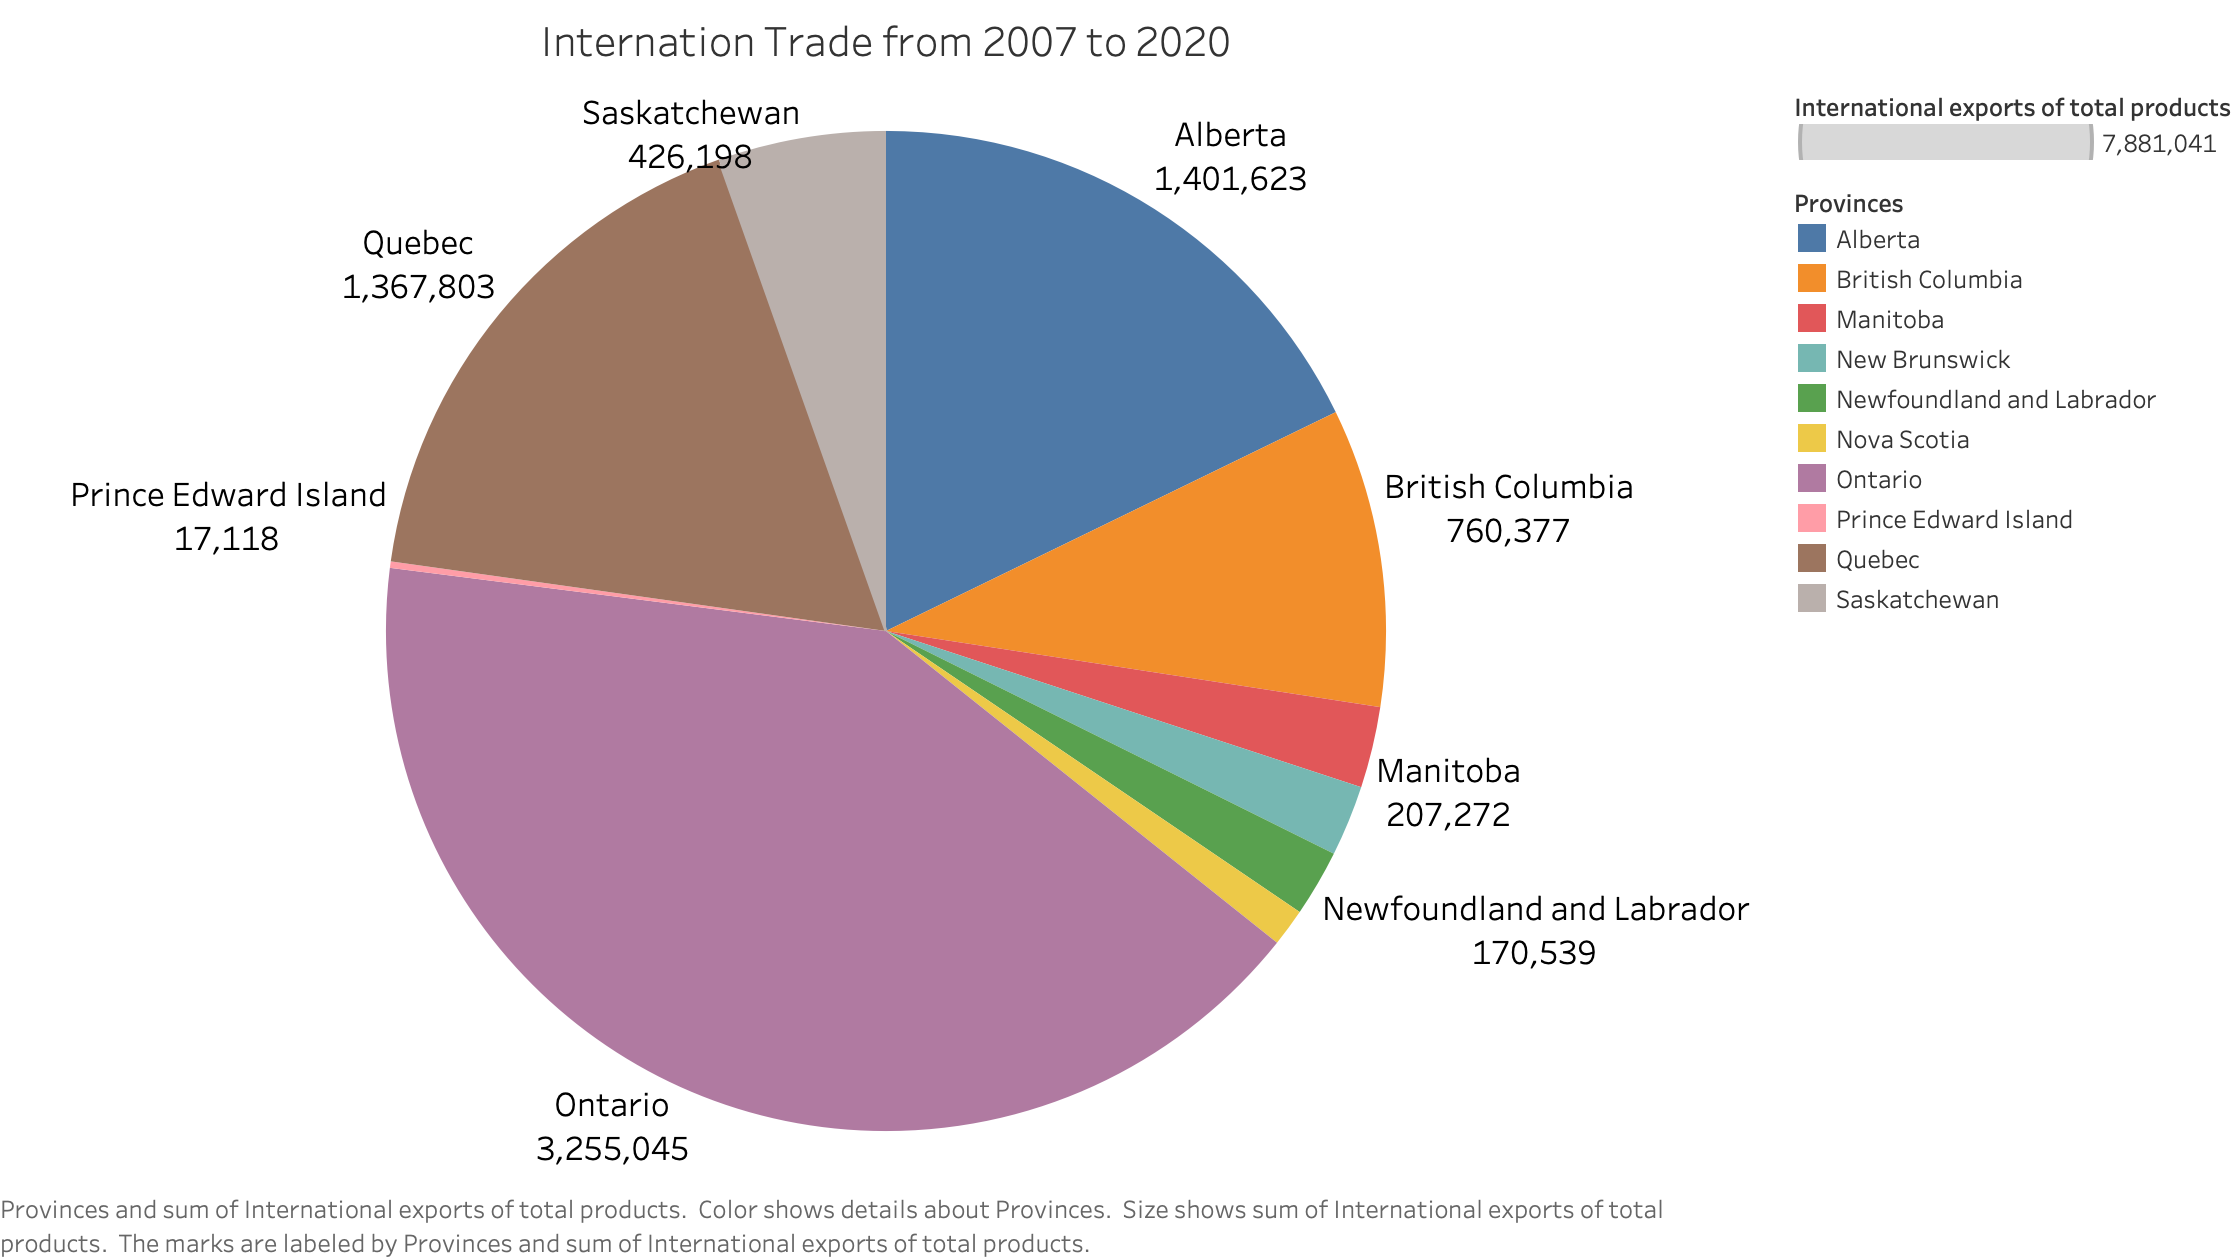
\includegraphics[width=1\linewidth]{Internatiol.png}
    \caption{Sum International Exports from 2007 to 2020}
    \label{fig:enter-label}
\end{figure}
\begin{figure}
    \centering
    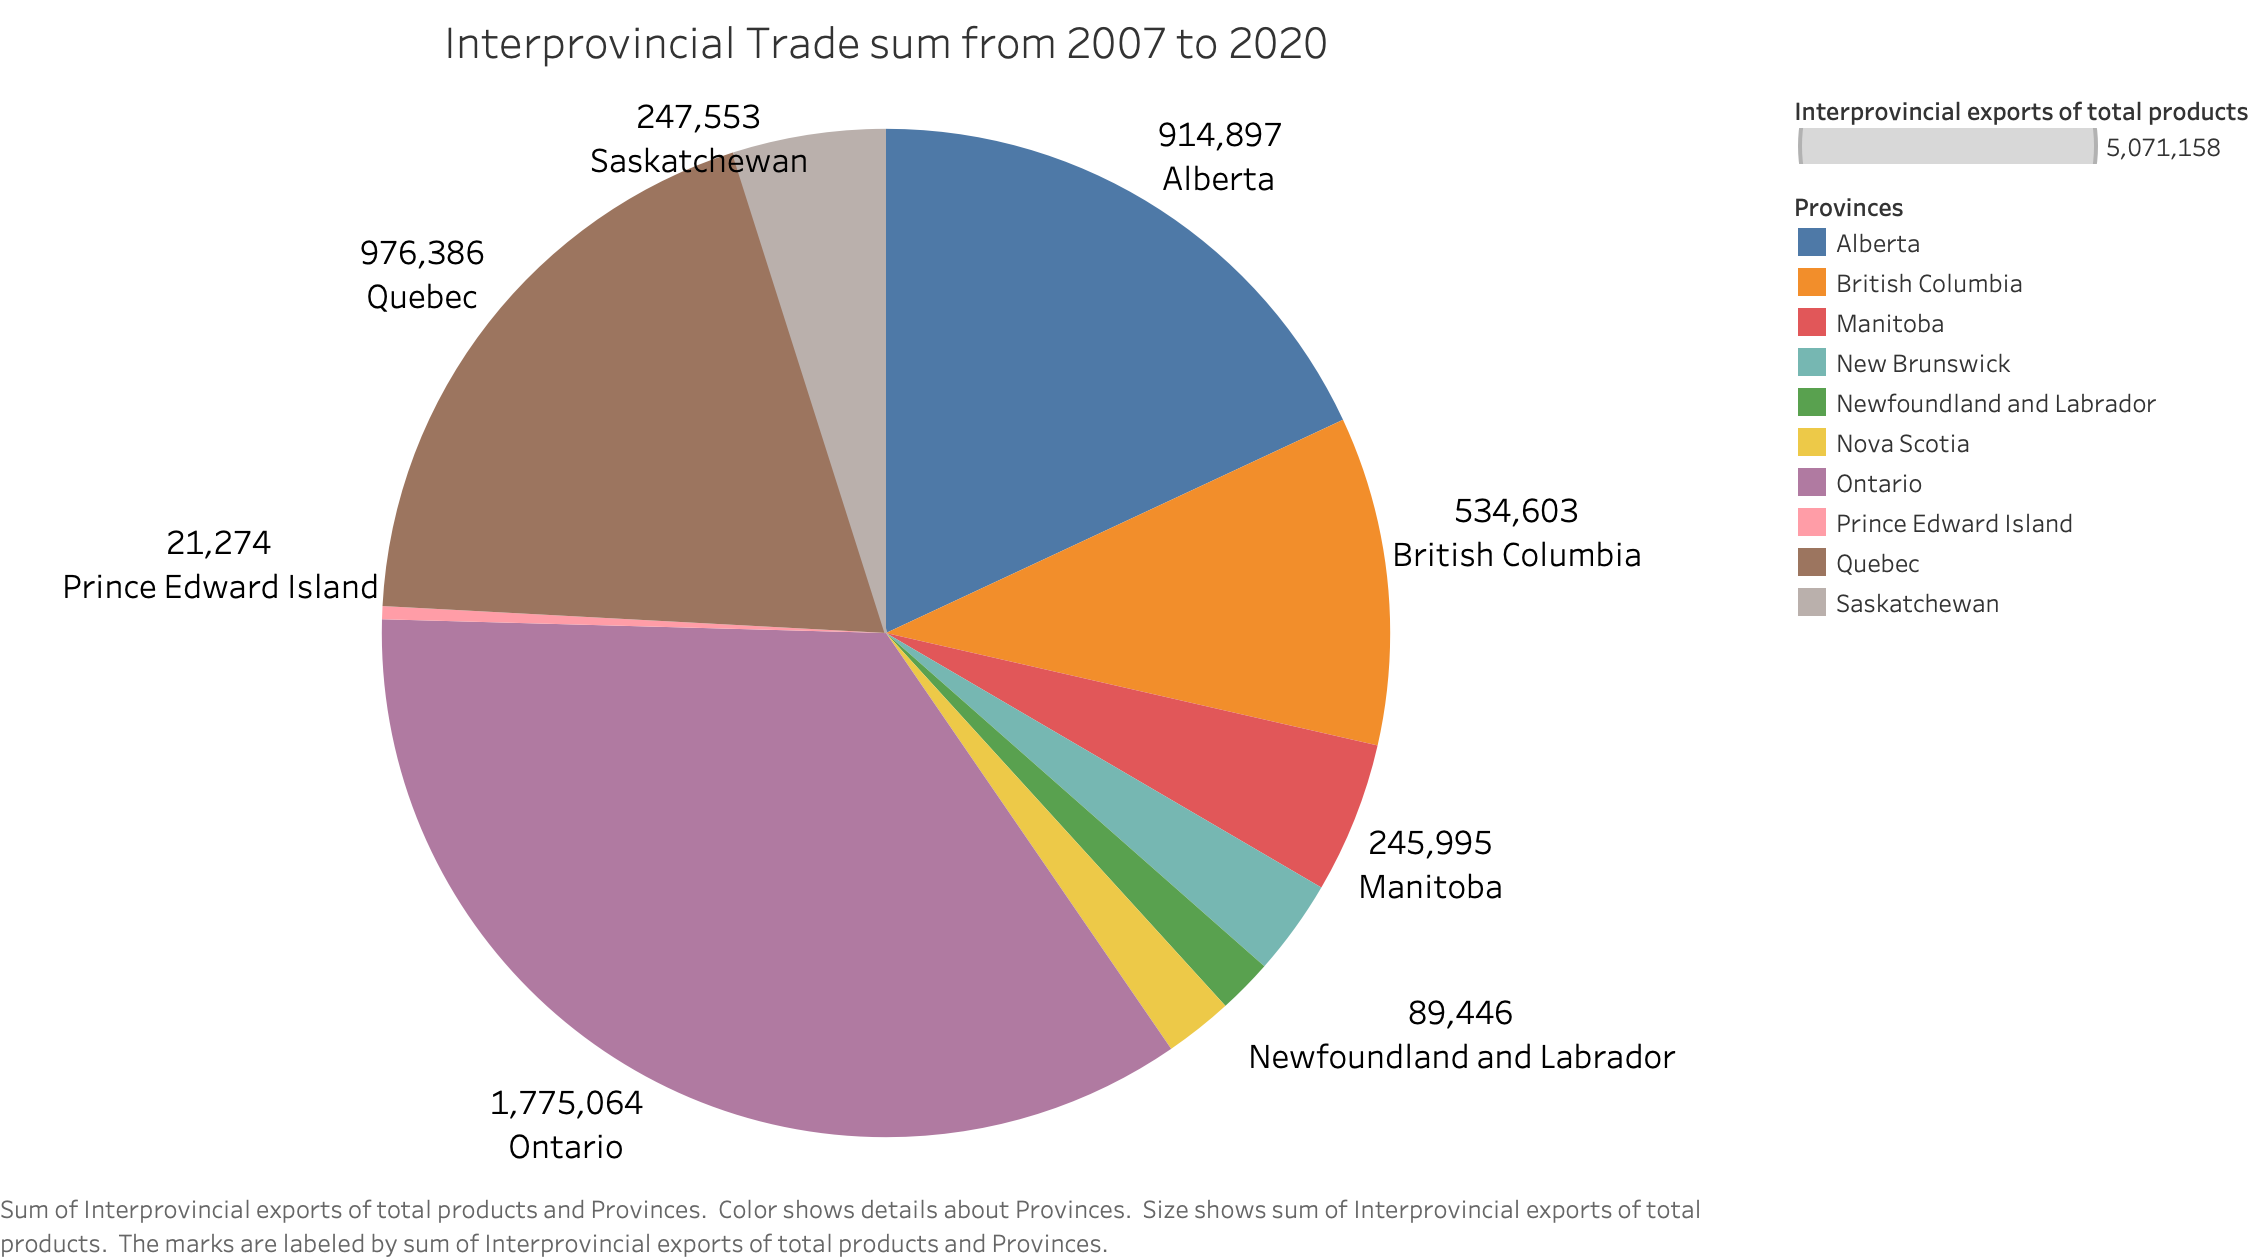
\includegraphics[width=1\linewidth]{Sheet 2.png}
    \caption{Sum Inter-provincial trade sum from 2007 to 2020}
    \label{fig:enter-label}
\end{figure}
\newpage
\section*{Trend Analysis}
We will now see how over time this relationship has changed and who has dominated international trade and inter-provincial trade.{fig:3}.
Looking at the trend for inter provincial exports and international exports by provinces reveals that Ontario has always dominated all provinces when it comes to both international and inter provincial trade . 
We can also see visually through the graph that international and inter provincial trade follow a similar path 
\subsection*{Ontario's Trade Dominance}
Ontario's significant role in Canada's trade, both internationally and interprovincially, can be attributed to several factors:
\begin{itemize}
    \item Large population (approximately 38\% of Canada's total)
    \item Strong industrial base
    \item Strategic location near the US border
    \item Well-developed infrastructure
\end{itemize}

\subsection*{The Gravity Model of Trade}
The gravity model predicts that trade between two entities (countries, provinces, etc.) is proportional to their economic sizes and inversely proportional to the distance between them. In its basic form:

\begin{equation}
    \text{Trade}_{ij} = G \cdot \frac{\text{GDP}_i \cdot \text{GDP}_j}{\text{Distance}_{ij}^2}
\end{equation}
While the basic gravity model explains much of Ontario's trade dominance, other factors also play roles:
\begin{itemize}
    \item Historical economic development
    \item Trade policies and agreements
    \item Industrial specialization
    \item Cultural and linguistic ties (especially relevant for Quebec)
\end{itemize}
\begin{figure}
    \centering
    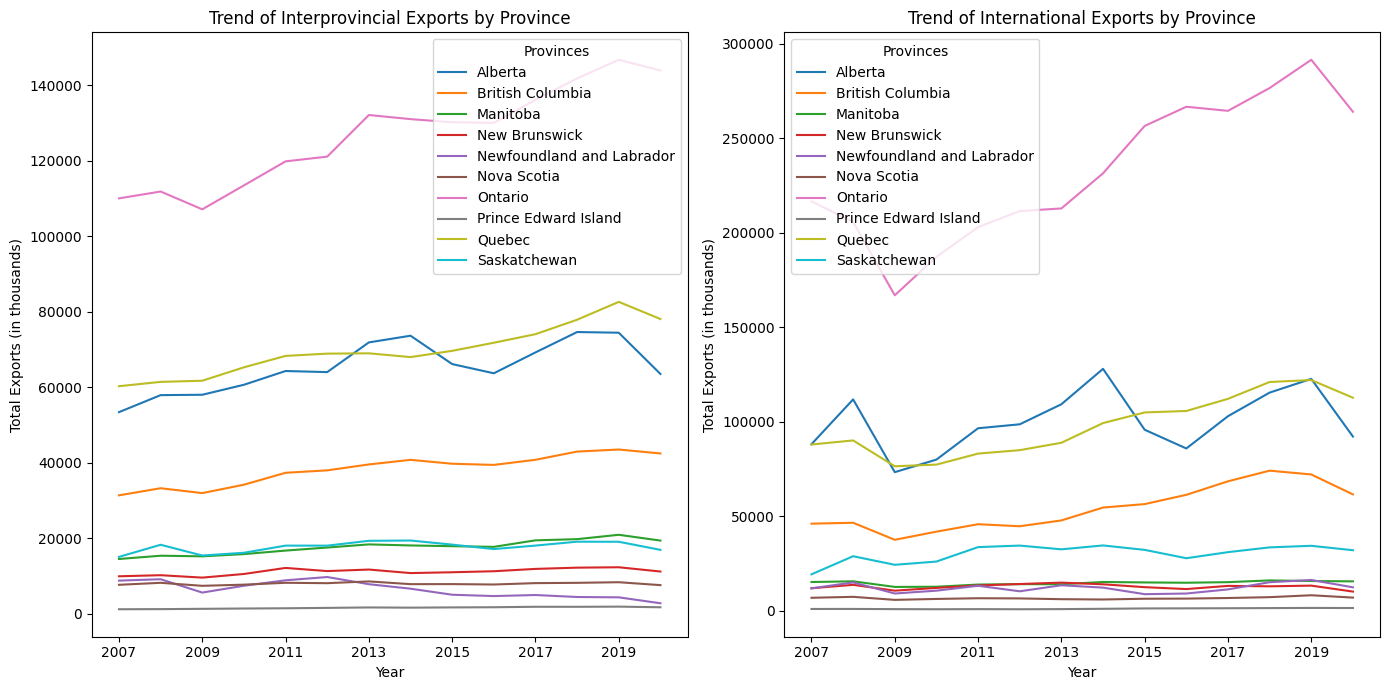
\includegraphics[width=1\linewidth]{timeseries.png}
    \caption{Time series: 2007 to 2020}
    \label{fig:enter-label}
\end{figure}
\section*{Lagging  Provinces}{
Looking at the Pie chart as well as the Time series analysis we that the provinces that more or less are stagnant in both international and inter-provincial trade are : 
\begin{itemize}
    \item Prince Edward Island
    \item Saskatchewan 
    \item Nova Scotia 
    \item Manitoba 
    \item Newfound land and Labrador 
\end{itemize}
\begin{figure}
    \centering
    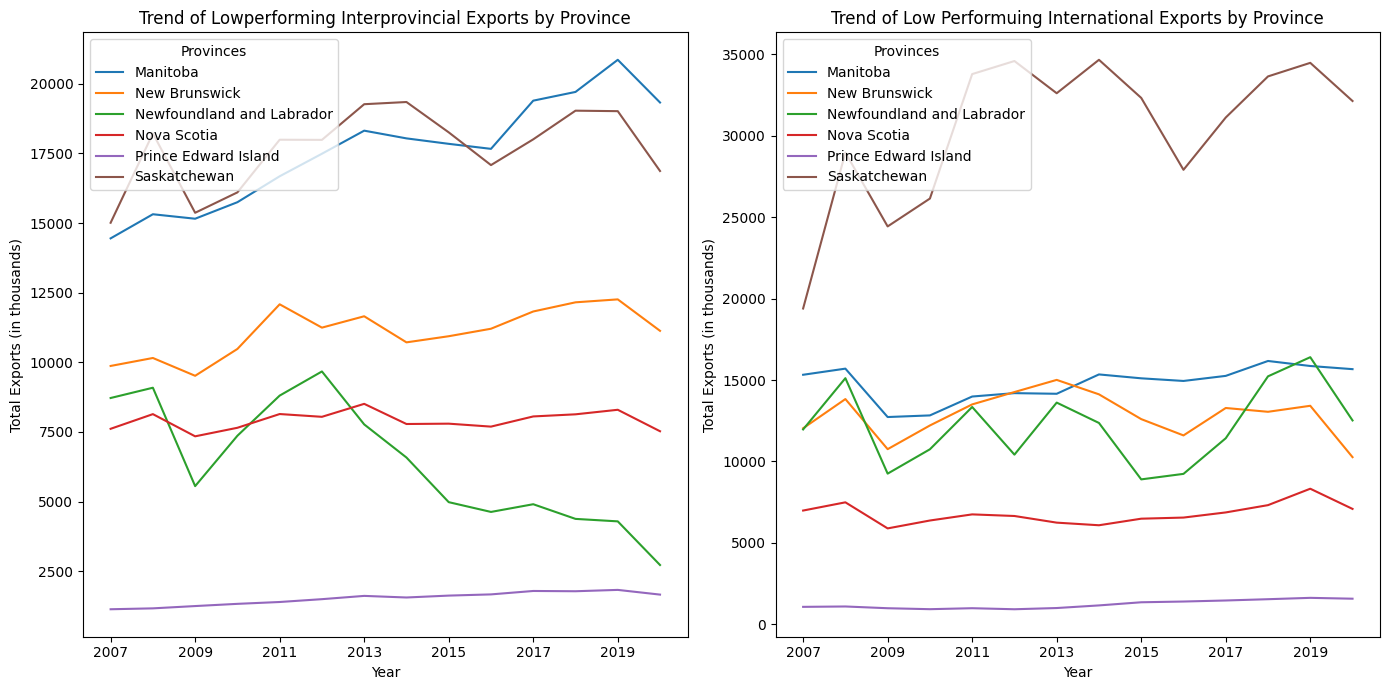
\includegraphics[width=1\linewidth]{image.png}
    \caption{Low performing provinces}
\end{figure}

}
\newpage
\section*{ Main Results}{
\subsection*{OLS regression model}{
The R-squared value is 0.969, indicating that international exports explain 96.9\% of the variance in inter-provincial exports.
The coefficient for international exports (0.5423) is statistically significant (t-statistic: 65.345, p-value: 0.000), suggesting a positive relationship between global and inter-provincial exports.
For every 1 unit increase in international exports, inter-provincial exports increase by 0.5423 units, on average. The high condition number (1.15e+05) suggests potential multicollinearity issues, meaning the explanatory variables (in this case, international exports) may be correlated with each other
The constant term (5696.8962) is also statistically significant, representing the expected inter-provincial exports when international exports are zero.
}


\begin{table}[htbp]
\centering
\caption{OLS Regression Results: Interprovincial Exports of Total Products}
\label{tab:ols_results}
\begin{tabular}{lcc}
\toprule
\textbf{Variable} & \textbf{Coefficient} & \textbf{Standard Error} \\
\midrule
Constant & 5696.8962*** & 742.233 \\
 & (7.675) & \\
International exports of total products & 0.5423*** & 0.008 \\
 & (65.345) & \\
\midrule
Observations & \multicolumn{2}{c}{140} \\
R-squared & \multicolumn{2}{c}{0.969} \\
Adjusted R-squared & \multicolumn{2}{c}{0.968} \\
F-statistic & \multicolumn{2}{c}{4270.0} \\
Prob (F-statistic) & \multicolumn{2}{c}{1.09e-105} \\
Durbin-Watson & \multicolumn{2}{c}{0.422} \\
\bottomrule
\multicolumn{3}{l}{\textit{Note:} t-statistics in parentheses} \\
\multicolumn{3}{l}{*** p<0.01, ** p<0.05, * p<0.1} \\
\end{tabular}
\end{table}

\newpage
\section*{Policy Recommendation}{
Looking at the lowest-performing provinces one has to look at all factors which are unique to these provinces affecting their trade. If we choose to dive into those our paper will become too complex and no concrete stance will be proposed.
But at the essence of all rational economics lie the factors of production land labor capital and entrepreneurship. of which the latter will be a key in boosting both inter-provincial and international trade.
The one factor that separates the front-running provinces from the laggard provinces is new enterprises. To produce final goods and to increase net value added in all these smaller provinces entrepreneurship is very important. Canada is a federation. The central government can give incentives to the service sector and the IT sector to move to these provinces. This will elevate the housing crisis in front-running provinces and help the smaller provinces grow. Moreover, the presence of IT companies will diversify the trade mix of these provinces (Statistics Canada, 2023) which is mainly based on agriculture raw materials processing and light/heavy manufacturing. This will protect these smaller provinces from cyclical commodities shocks(Buyuksahin, 2016, p. 1).
To achieve all mentioned above a good labor force is also needed that will have the skills to promote industry. Out-migration also becomes an issue. Which leads to brain drain. Newcomers to Canada in the productive age should be encouraged to move and settle in these provinces and disincentives to move out. 
}
\newpage
\section*{Conclusion}{
International Trade by Canadian Provinces Complement Their Interprovincial trade
The policy recommendations made are very common and general. Any person could have made it. To make a solid policy recommendation one has to look deep into the issues of every province. Look at the trade mix look that the industries in that province and set incentive structures in a way that they cannot be exploited.

}


\newpage
\section*{Random Forest model }{
\textbf{R2 Score}: 0.9751760879099278 \newline The R2 score, also known as the coefficient of determination, indicates how well the model explains the variance in the target variable. An R2 of 0.9752 is excellent, suggesting that the Random Forest model explains about 97.52\% of the variance in inter-provincial exports. This is a very high value, indicating that the model fits the data extremely well too well it is overfitting.
A high R-squared value can often be a red flag for overfitting in a model.
\par
 Random Forest inherently assumes independence between observations. While lagged features capture some dependencies, more sophisticated techniques like recurrent neural networks might better suit complex time series patterns.
 \par
\textbf{ Mean Squared Error}: 34875959.783368394

}

\begin{figure}
    \centering
    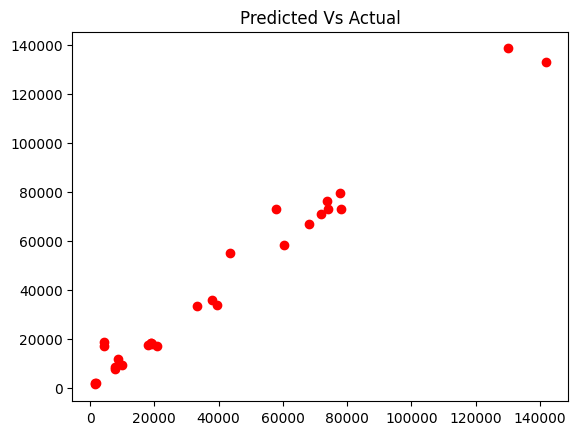
\includegraphics[width=0.5\linewidth]{rfoverfit.png}
    \caption{Classic Overfit}
    \label{fig:enter-label}
\end{figure}

\newpage
\begin{thebibliography}{4}

\bibitem{StatCanTrade}
Statistics Canada. (2024). Table 12-10-0088-01 Interprovincial and international trade flows, basic prices, summary level (x 1,000,000). \url{https://www150.statcan.gc.ca/t1/tbl1/en/tv.action?pid=1210008801}

\bibitem{Buyuksahin2016}
Buyuksahin, B. (2016). The impact of oil price shocks on the Canadian economy. \textit{Bank of Canada Review}, Autumn 2016, 1-14.

\bibitem{StatCanBalanceSheet}
Statistics Canada. (2023, May 15). Canada's national balance sheet, first quarter 2023. \url{https://www150.statcan.gc.ca/n1/daily-quotidien/230501/dq230501a-eng.htm}

\bibitem{StatCanPopulation}
Statistics Canada. (2024). Population estimates, quarterly. \url{https://www150.statcan.gc.ca/t1/tbl1/en/tv.action?pid=1710002201&pickMembers%5B0%5D=1.10&cubeTimeFrame.startYear=2018+/+2019&cubeTimeFrame.endYear=2022+/+2023}

\end{thebibliography}
\end{document}

